Teorię kopuł zapoczątkował Abe Sklar w \cite{Sklar_Theorem}, podając następujące twierdzenie:

\begin{thm}[Twierdzenie Sklara]
	Niech $X_1, X_2, \dots, X_d$ będą zmiennymi losowymi ciągłymi, o dystrybuantach $F_1, \dots, F_d$, i rozkładzie łącznym z dystrybuantą $F$. Wtedy istnieje dokładnie jedna \emph{kopuła} $C$, taka że dla wszystkich $\mathbf{x} = (x_1, \dots, x_d) \in \mathbb{R}^d$:
	\begin{equation}
		F(x_1, \dots, x_d) = C(F_1(x_1), \dots, F_d(x_d)).
		\label{eq:sklar_theorem}
	\end{equation}
	
	Zachodzi również twierdzenie odwrotne: Mając dowolne dystrybuanty $F_1, \dots, F_d$ i kopułę $C$, funkcja $F$ zdefiniowana według \ref{eq:sklar_theorem} jest d-wymiarową dystrybuantą, o rozkładach brzegowych $F_1, \dots, F_d$. 
	\label{thm:sklar_theorem}
\end{thm}

Twierdzenie \ref{thm:sklar_theorem} przede wszystkim podaje więc algorytm postępowania mówiący w jaki sposób otrzymać wielowymiarowy rozkład o dowolnie wybranych, potencjalnie różnych rozkładach brzegowych. Dodatkowo, Sklar stwierdza istnienie pewnego obiektu, nazwanego kopułą/funkcją łączącą (łac.\emph{copulae}: łączyć) który jest jednoznacznie zdefiniowany dla dowolnego ciągłego rozkładu wielowymiarowego, w taki sposób, że rozkład łączny da się przedstawić jako tę funkcję zaaplikowaną do rozkładów brzegowych.\\

Oczywistym jest, że nie wszystkie wielowymiarowe funkcje mogą pełnić taką rolę. Rozważymy więc jakie warunki musi spełniać $C$ z twierdzenia \ref{thm:sklar_theorem}, aby mogła być kopułą.
\begin{df}[Grounded function]
	Rozważmy $A_1$ i $A_2$ - dwa niepuste podzbiory $\mathbb{R}$, oraz funkcję $G\colon A_1\times A_2\mapsto\mathbb{R}$. Niech $a_i$ oznacza najmniejszy element $A_i$, dla $i=1, 2$. Funkcję $G$ będziemy nazywać uziemioną (\emph{grounded}), jeśli dla każdej pary $(v, z)$ z $A_1\times A_2$,
	\begin{equation}
		G(a_1, z) = 0 = G(v, a_2).
	\end{equation}
	\label{def:grounded_function}
\end{df}

\begin{df}[2-increasing function]
	$G\colon A_1\times A_2\mapsto \mathbb{R}$ nazywamy dwu-rosnącą (\emph{2-increasing}), jesli dla każdego prostokąta $[v_1, v_2]\times [z_1, z_2]$ $(v_1 \leqslant v_2$, $z_1\leqslant z_2)$ którego wierzchołki leżą w $A_1 \times A_2$ mamy
	\begin{equation}
		G(v_2, z_2) - G(v_2, z_1) - G(v_1, z_2) + G(v_1, z_1) \geqslant 0.
	\end{equation}
	\label{def:two_increasing_function}
\end{df}

Definicje \ref{def:grounded_function} oraz \ref{def:two_increasing_function} pozwalają na poprawne zdefiniowanie kopuły:
\begin{df}[Dwuwymiarowa kopuła]
	Dwuwymiarową kopułą $C$ nazwiemy funkcję rzeczywistą zdefiniowaną na kwadracie jednostkowym:
	$$ C\colon [0, 1]\times[0, 1] \mapsto \mathbb{R},$$ o następujących własnościach:
	\begin{itemize}
		\item uziemiona $\big(C(v, 0) = 0 = C(0, z)\big)$
		\item dwu-rosnąca
		\item $C(v, 1) = v$ oraz $C(1, z) = z$ dla wszystkich $(v, z)\in [0,1]\times [0, 1].$
	\end{itemize}
	\label{def:bivariate_copula}
\end{df}

Aby zrozumieć czym kopuła tak naprawdę jest warto wrócić do twierdzenia \ref{thm:sklar_theorem}. Równość \ref{eq:sklar_theorem} implikuje, że kopuła musi być dystrybuantą pewnego wielowymiarowego rozkładu. Definicja kopuły w \ref{def:bivariate_copula} mówi natomiast, że ta dystrybuanta jest zdefiniowana na \emph{kwadracie jednostkowym}. Kopuła jest więc niczym innym jak dystrybuantą wielowymiarowego rozkładu jednostajnego. Istotnie: można pokazać, że argumenty kopuli w równaniu \ref{eq:sklar_theorem} mają rozkład jednostajny, co udowadniamy poniżej i ilustrujemy na rysunku \ref{fig:PIT}.

\begin{df}[Probability integral transform]
	Jeśli $X\sim F$ jest ciągłą zmienną losową, a $x$ jest jej realizacją, to transformację $u\coloneqq F(x)$ nazywamy \emph{probability integral transform} (PIT) w punkcie $x$.
	\label{def:PIT}
\end{df}
\begin{thm}[Probability integral transform]
	Jeśli $X\sim F$ jest ciągłą zmienną losową, to $U\coloneqq F(X)$ ma rozkład jednostajny.
\end{thm}
\begin{proof}
	$$P(U\leqslant u) = P(F(X) \leqslant u) = P(X\leqslant F^{-1}(u))=F(F^{-1}(u))=u.$$
\end{proof}

\begin{figure}[H]
	\centering
	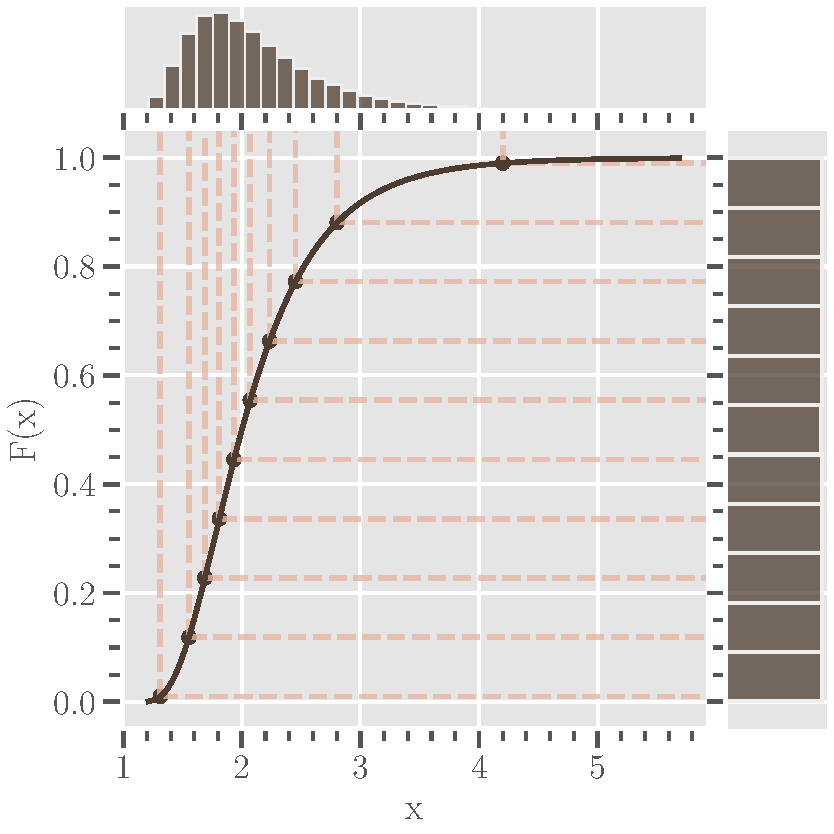
\includegraphics[width=0.6\linewidth]{01_PIT}	
	\caption{\textbf{Probability Integral Transform. } Ilustracja działania PIT. Zmienna losowa z rozkładu lognormalnego $
		\mathcal{LN}(0.5, 1)$ (pozioma oś) przekształcana jest przez własną dystrybuantę do rozkładu jednostajnego $\mathcal{U}(0, 1)$ (pionowa oś).\label{fig:PIT}}
\end{figure}

Wróćmy na chwilę do oryginalnego pytania, czyli modelowania wielowymiarowych zmiennych losowych. Na początku rozdziału zdefiniowaliśmy kopułę jako funkcję spełniającą równanie \ref{eq:sklar_theorem} z twierdzenia Sklara, czyli:
$$F(x_1, \dots, x_d) = C(F_1(x_1), \dots, F_d(x_d)).$$

Prawą stronę równania stanowią wyizolowane rozkłady brzegowe, oraz pewna funkcja $C$, postać której jest kompletnie od nich niezależna. Lewa strona równania, to natomiast rozkład łączny pewnej zmiennej losowej. Jeśli zastanowimy się co wpływa na charakter rozkładu łącznego zmiennej losowej, dojdziemy do wniosku, że istnieją dwa komponenty: zachowanie rozkładów brzegowych, oraz ich współzależności. Biorąc znów pod uwagę prawą stronę równania, kopuła musi więc odpowiadać za współzależności między rozkładami brzegowymi. \\
Istotnie, kopuły pozwalają na rozdzielenie problemu modelowania rozkładu łącznego, na modelowanie osobno rozkładów brzegowych, a osobno struktury ich współzależności (\cite{Sklar_Theorem}, \cite{Joe_Multivariate_Models}). Ta pozorna prostota tworzenia wielowymiarowych modeli przyczyniła się do szybkiej ich popularyzacji, ale i przyniosła ze sobą duże ryzyko modelu. Najbardziej znanym tego przykładem jest zapewne fiasko modeli wyceniających produkty typu CDO (\cite{CDS_Copula}), które niedoszacowywały nasilenia korelacji bankructw wewnątrz struktury tego kontraktu.\\

Możliwość dokonania takiej dekompozycji implikuje, że zależność zmiennych losowych $X$, $Y$ daje się przedstawić jedynie w terminach łączącej je kopuły $C$. Z tego powodu, interesujące są dla nas miary zależności które są niezmiennicze na monotonicznie rosnące przekształcenia zmiennych losowych.

\begin{df}[Miara zgodności]
	Niech $\mathcal{R}$ będzie przestrzenią ciągłych rozkładów łącznych, oraz $(X, Y) \in \mathcal{R}$ wektorem losowym z tej przestrzeni. Niech $C$ oznacza kopułę łączącą rozkłady brzegowe $X$ i $Y$. Miarą zgodności $M_{X,Y}$ (alternatywnie: $M_C$) między $X$ a $Y$ nazwiemy funkcję $M_{X,Y}\colon \mathcal{R}\mapsto A\subset\R$ wtedy i tylko wtedy gdy spełnia aksjomaty:
	\begin{enumerate}
		\item Dziedziny: jest zdefiniowana dla dowolnego wektora zmiennych losowych $(X, Y) \in \mathcal{R}$
		\item Symetrii: $M_{X,Y}=M_{Y,X}$
		\item Zgodności: jeśli $C_1(u,v) \leqslant C_2(u,v)$ dla wszystkich $(u, v)\in[0,1]^2$, to $M_{C_1} \leqslant M_{C_2}.$
		\item Zbioru wartości: $M_{X,Y}\in[-1,1]$
		\item Niezależności: $X$ i $Y$ są niezależne, to $M_{X,Y}=0$
		\item Zmiany znaku: $M_{-X,Y}=M_{X,-Y}=-M_{Y,X}$
		\item Ciągłości: jeśli $\{(X_n,Y_n)\}$ jest ciągiem ciągłych zmiennych losowych o kopułach $\{C_n\}$, oraz 
		$$ \lim\limits_{n\to\infty} C_n(u, v) =C(u, v)\text{, dla każdych }(u, v)\in[0,1]^2,$$
		to wtedy
		$$ \lim\limits_{n\to\infty}M_{X_n,Y_n}=M_{X,Y}.$$
	\end{enumerate}
	\label{def:miara_zgodnosci}		
\end{df}
Aksjomatyczne podejście z definicji \ref{def:miara_zgodnosci} zawęża przestrzeń miar zgodności do takich, które są niezmiennicze względem rosnących transformacji, czyli:
$$ M_{X,Y} = M_{\alpha(X), \beta(Y)},$$
dla dowolnych funkcji $\alpha,\beta$ rosnących prawie wszędzie. Użycie takich miar w teorii kopuł wydaje się być naturalnym wyborem - ponieważ pozostaną one takie same zarówno dla zmiennych oryginalnych, jak i dla zmiennych przetransformowanych poprzez \ref{def:PIT}, zgodnie z  definicją \emph{PIT}.\\